\documentclass[a4paper,11pt]{article}

\usepackage{graphicx}
\usepackage[printwatermark]{xwatermark}
\usepackage[margin=1in]{geometry}
\usepackage[doublespacing]{setspace}
\usepackage{color} % needed if you use xfig graphics at all
\usepackage{xcolor}
\usepackage{url}
\usepackage{hyperref}
\usepackage{csquotes}
\usepackage{listings}
\usepackage{courier}
\usepackage{subfigure}
\usepackage{mdwlist}
\usepackage{tabu}
\usepackage{array,etoolbox}
\usepackage{lscape}
\usepackage{rotating}
\usepackage[toc,page]{appendix}
\usepackage{pdfpages}
\usepackage{pdflscape}	%allows landscape orientation for floats
\usepackage{afterpage}
\usepackage{ragged2e}
\usepackage{textcomp}
\usepackage{mdwlist}
\usepackage{amsmath}	% allows \text{} in math mode $$ or \[ \]
\usepackage{amsthm}		%used for defining theorems
\usepackage{longtable} % for 'longtable' environment




\author{Fraser Brown}
%\institute{Heriot-Watt University}
\date{\today}

\graphicspath{{../figures/}}

\begin{document}

%Title
\begin{titlepage}
   \vspace*{\stretch{1.0}}
   \begin{center}
      \Large\textbf{Digital Forensics Masterclass Labsheet}\\
      \large\textit{File System Forensics}
   \end{center}
   \vspace*{\stretch{2.0}}
\end{titlepage}

\tableofcontents
\newpage

\section{Lab Overview}
The learning objective for this lab is for participants to gain practical experience in digital forensics specifically file system analysis. During the lab you will gain experience in the following tools, environments and tasks:
\begin{itemize*}
	\item Kali Linux\footnote{https://www.kali.org/}
	\item The Sleuth Kit (TSK)\footnote{https://www.sleuthkit.org/} file system analysis tool kit.
	\item Forensic image creation.
	\item Identifying Attributes about file systems (data uni size file type).
	\item Deleted file recover procedure.
	\item Searching for evidence on a file system.
	\item Event timeline creation?????
\end{itemize*}

As an \textit{optional} bit of fun for the lab, we will be adding a capture the flag (CTF) style element. For each task there is a set goal, that may be finding a word or phrase in unallocated space, the hash of a recovered file etc. After each task is completed please enter the given evidence as an argument to the \texttt{flagfound} script as follows:\\
\verb|$  ./flagfound "YOUR EVIDENCE HERE"|


\section{Removable Media Resource Credits}
The USB resources we will be using in today's lab are from the National Institute of Standards and Technology (NIST) as part of their Computer Forensic Reference Data Sets (CFReDS)\footnote{https://www.cfreds.nist.gov/}.  We will be focusing on a subsection of this case using ``Removable Media {\#}2'', in order to investigate material covered in the lecture. The scenario section below will set the scene. 
 
 If you are interested in exploring this scenario more the whole case can be fond here:\\
 \verb|https://www.cfreds.nist.gov/data_leakage_case/data-leakage-case.html|

\section{Environment Setup}
\subsection*{Installing Kali Linux in Virtual Box}
Before your digital investigation can begin you are required to create a lab environment, for this we will be using a virtual machine (VM) instance of Kali Linux.
Your user accounts should have been given access to virtual box in the university lab (EM2.50). We are using a virtual machine to no only give you complete control over the operating system, but so this lab can be carried out safely. Below we will show you how to create a Kali Linux VM.
	\begin{enumerate*}
	 \item Open a terminal window and enter the following command to open Virtual Box:\\
		\texttt{{\$}	virtualbox {\&}}
	\item Return to the terminal window and follow \texttt{LoadingKaliVM.pdf} instructions, created by Mike Just.
	\item Start your Kali VM
	\end{enumerate*}
	
\section{Kali Linux Login Information}
	 username: \texttt{root}
	 password: \texttt{toor}

\subsection{Note About Root}
In Kali Linux you are logged in as the root user of the system, therefore the operating system assumes you know what you are doing. Double check the commands you are entering especially if they are related to \texttt{rm}.

\subsection{Create a Case Directory for Investigation}
Within your home directory create the a \texttt{cases} directory and inside that create a directory called \texttt{001} to represent the case number you are working on. Make this your current working directory in a terminal window.

\newpage
\section{Task 1: Create a Forensic Image}
There should be USB flash drives available for this lab, with the removable media evidence on them.  In this lab we will be working with .dd images also known as raw images. There are many tools available to create the a forensic image with Kali Linux comes installed with both GUI and command line versions. It is up to you which you use however I would recommend \texttt{Guymager}.\\

\textbf{NOTE:} \textit{Sadly we were not able to attain writeblockers for this lab, please remember that writeblockers are important for prevention of unwanted meta data changes to media by the investigators operating system. Writeblockers are used in industry when creating forensic images of a system.}\\

Insert USB Stick into computer and confirm it has been recognised by the Kali Linux VM, you can check this in either in files that a usb device is visable in the left hand pane or by running \texttt{df -h} in the command line and checking for a 4GB device located in \texttt{/media/root/}. \\

Open a terminal window (we will use this later anyway) and enter: \texttt{guymager {\&}} the following GUI should appear:
\begin{figure}[h]
	\centering
	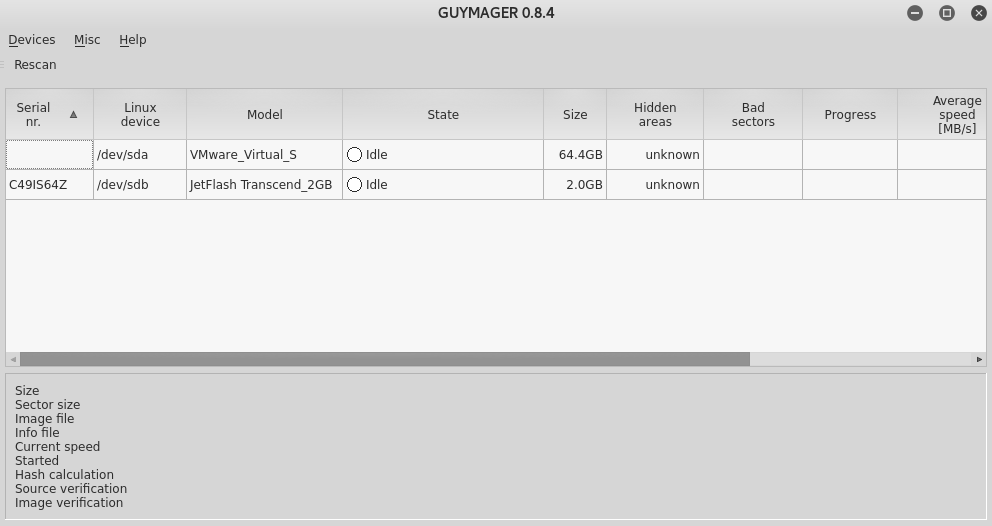
\includegraphics[scale=0.5]{guymager-window}
	\caption{\textit{guymager gui window example}}
	\label{fig:guymager-main-window}
\end{figure}
\\
If the 4GB usb drive does not show up press \texttt{f5} to rescan devices. From here you can select the drive you wish to create an image of, right click the 4GB drive and select the \texttt{Aquire image} option. Fill out the guy form making sure you have the following options then click start:
\begin{itemize*}
\item Linux dd raw image
\item Uncheck split image
\item Destination is set to \texttt{/home/cases/001/image/}
\item Image filename set to \texttt{revmed2}
\item Info filename set to \texttt{revmed2}
\item Check calculate md5 hash
\item Check verify image after acquisition
\end{itemize*}
\begin{figure}
	\centering
	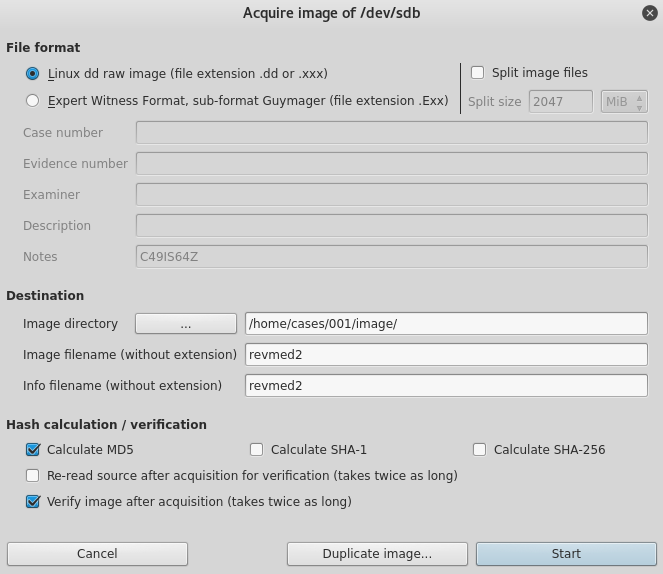
\includegraphics[scale=0.5]{guymager-aquisition-window}
	\caption{\textit{guymager acquisition window example}}
	\label{fig:guymager-aquisition-window}
\end{figure}

Once you have clicked start you shall be returned to the main guymager window and a progress bar should be displayed. once the progress bar states ``Finished - Verified {\&} ok'' your forensic image has been created. To confirm list the contents of \texttt{/home/cases/001/image/} in a terminal window, you should find the following files: 
\begin{itemize*}
\item \texttt{revmed2.dd} : the image file we can now perform analysis on.
\item \texttt{revmed2.info} : acquisition info such as cryptographic hash.
\end{itemize*}

\subsubsection*{Verify The Media Hash}
in order to confirm that our image is the same as the contents of the USB we must generate a hash of the .dd file and compare it to the hash listed in the .info file.
in a terminal window run the following:
\texttt{md5sum image/revmed2.dd}
the output should match the hash listed in the .info file you just created.

Remove the USB from your machine and return it to the evidence box.

\textit{\textbf{Optional:} enter the hash into the \texttt{findflag} program to receive your first flag.}

\section{Task 2: File System Information Gathering using TSK}
Now that we have a forensic image we can start to analyse the evidence, using The Sleuth Kit (TSK).

Commands we will be using to gather information on the system
\begin{itemize*}
	\item \textbf{\texttt{mmls}}:\\ \texttt{mmls} displays the layout of the partitions in a volume system, which include partition tables and disk labels.
	\item \textbf{\texttt{fsstat}}:\\ \texttt{fsstat} displays the details associated with a file system. (requires partition starting point in sectors)
\end{itemize*}

\subsection*{Find the following Information:}
Using the tools above and files you currently have (.dd, .info) find the following information: (write it down you will need to reference it later)
\begin{enumerate*}
	\item what is the cluster size of the file system?
	\item what is the sector size of the file system?
	\item Given that a cluster contains consecutive sectors, how many sectors are in one cluster?
	\item What partition has content data in it?
	\item What is the staring point of the File System partition (in sectors)?
	\item Can you confirm the file system type is fat32 using a TSK tool or other information you have gathered (.info) file?
\end{enumerate*}


\section{Task 3: Searching Unallocated Space for Evidence}
Commands we will be using to gather information on the system
\begin{itemize*}
	\item \textbf{\texttt{blkls}}:\\ \texttt{blkls} opens the named image(s) and copies file system data  units  (blocks).   By default,  \texttt{blkls} copies the contents of unallocated data blocks. 
	\item \textbf{\texttt{fsstat}}:\\ \texttt{fsstat} displays the details associated with a file system. (requires partition starting point in sectors)
\end{itemize*}

\section{Task 4: Deleted File Recovery using Meta Data Pointers}
Your another member of your digital investigation team has mentioned there is something suspicious with a file called \texttt{progress/my\_friends.svg} that was removed from the file image, they have asked to to check if the deleted file is recoverable and verify the data is of format \texttt{.svg} then compare the recovered data to his found SHA1 hash.

{\noindent
\textbf{Co-Workers SHA1 hash:}\\
\texttt{95175c35be9d74ad3e271550e358e634154ba105  progress/my\_friends.svg}
}
\subsection*{Commands used in this task}
\begin{itemize*}
	\item \textbf{\texttt{fsstat}}:\\ \texttt{fsstat} Displays the details associated with a file system. (requires partition starting point in sectors).
	\item \textbf{\texttt{fls}}:\\ \texttt{fls} List file and directory names in a disk image, including its associated \textit{inode} number.
	\item \textbf{\texttt{istat}}:\\ \texttt{istat}  displays the uid, gid, mode, size, link number, modified, accessed, changed times, and all the \textit{disk units} a structure has allocated.
	\item \textbf{\texttt{blkstat}}: displays the allocation status of the given data unit. 
	\item \textbf{\texttt{blkls}}:\\ \texttt{blkls} opens  the named image(s) and copies file system data units (blocks).  By default, blkls copies the contents of unallocated data blocks.
	\item \textbf{\texttt{sha1sum}}: \texttt{sha1sum}	- compute and check SHA1 message digest
	
	\item \textbf{\texttt{icat}}: \\ \text{icat} Outputs the content of a file based on its \textit{inode} number according to the details in its meta data pointer.
	
	\item \textbf{\texttt{file}}: \text{file} - determine file type
\end{itemize*}

\subsection*{Talk Walkthrough}
{\noindent
\textbf{Task 4.1: List the names and inode info of all deleted files on the image:}\\
We are looking for a deleted file and have been given a name to find within this .dd image. We know that data in file systems have various pointers for metadata, one of which is a file name pointer. We can use TSK tools that proceed with an \texttt{f} in this instance we want to see all files that were deleted on the data partition, \texttt{fls} will let us do this.\\
\\
\verb|# fls -rd -o 128 [path-to-image]|\\

\noindent
\textbf{4.1 Questions:}
\begin{enumerate*}
	\item What is the \textit{iNode Address} for this \texttt{my\_friends.svg}?\\
\end{enumerate*}
}

{\noindent
\textbf{Task 4.2: Based on the inode for my\_friends.svg extract stats on it:}\\
Using this inode (meta data) pointer, we can gather stats on the data units in question using \texttt{istat}.\\
\verb|# istat -o 128 [path-to-image]  1651335|\\

\noindent
\textbf{4.2 Questions:}
\begin{enumerate*}
	\item What is the file size of the Image?
	\item What sector does the data unit start at?
	\item what sector does the data unit end at?\\
\end{enumerate*}	
}
{\noindent
\textbf{Task 4.3: Get clusters sectors are in:}\\
\verb|# blkstat -o 128 [path-to-image]  111408|\\
\noindent
\verb|# blkstat -o 128 [path-to-image]  111522|\\

\noindent
\textbf{4.3 Questions:}
\begin{enumerate*}
	\item What is difference between start and end clusters?\\
\end{enumerate*}	
}
{\noindent
\textbf{Task 4.4: Recover those sectors from unallocated space:}\\
Given we now know the start and end sectors and have verified that their clusters are not overwritten with other data, we can begin the recovery process.
\texttt{blkls} will extract all unallocated data units between a given start and end point and write it to a new file (if no points are given it will gather all unallocated space). 

\verb|# blkls -o 128 [path-to-image] > output/recovered-file.blkls|
}\\

{\noindent
\textbf{Task 4.4: Calculate hash for recoveredfile.blkls:}\\
We have successfully recovered the requested file now verify that its hash matches the one our co-worker found as follows:
\verb|# sha1sum output/recovered-file.blkls|
}\\

{\noindent
Verify it is a \texttt{.svg} file with the file command:\\
\textbf{Task 4.5: Check the file type of the recovered data units:}\\
\verb|# file output/recoved-file.blkls|\\

\textbf{4.5 Questions:}
\begin{enumerate*}
	\item What is actual type of the file?
	\item Do you know why the file extension contradicts the actual type?\\
\end{enumerate*}	
}

\end{document}